\documentclass{subfile}

\begin{document}
  \section{Analysis on SIR, SIRS, SIS Epidemic Models}
  \subsection{SIR Model}
  From the simulation result, there exists an inversly proportional relationship between \(p\) and termination of the epidemic. While the number of infected is proportional \(p\). The relationship between \(p\) and termination of epidemic or the number of infected is also non-linear by observation from simulation result.
  \begin{tabular}{cc}
    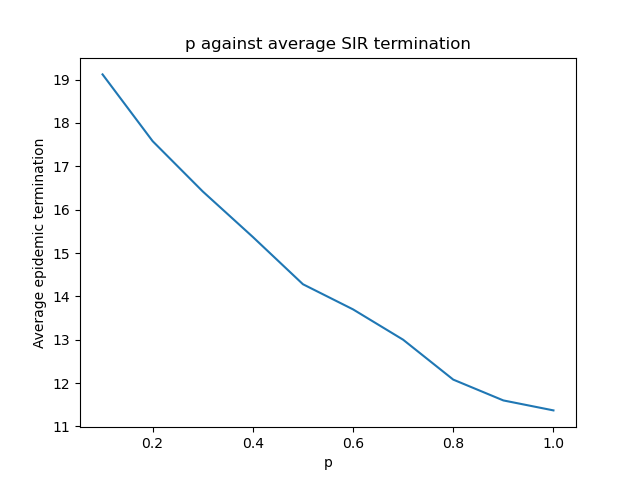
\includegraphics[scale=0.5]{p_sir_t} & 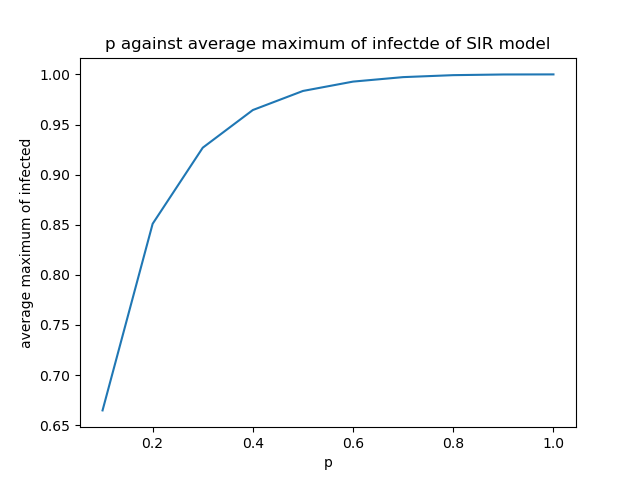
\includegraphics[scale=0.5]{p_infect_sir}\\
  \end{tabular}

  Further more, we can observe an linear increase in the termination of the SIR epidemic when \(i\) increased.
\end{document}
